% Copyright 2004 by Till Tantau <tantau@users.sourceforge.net>.
%
% In principle, this file can be redistributed and/or modified under
% the terms of the GNU Public License, version 2.
%
% However, this file is supposed to be a template to be modified
% for your own needs. For this reason, if you use this file as a
% template and not specifically distribute it as part of a another
% package/program, I grant the extra permission to freely copy and
% modify this file as you see fit and even to delete this copyright
% notice. 

\documentclass{beamer}
\usepackage{amsmath,bm}
\usepackage{tikz}
\usetikzlibrary{arrows,automata}
\usepackage{graphicx}

\newcommand{\ssquare}{\text{\scalebox{0.6}{$\square$}}}
\newcommand{\U}{\bm{\mathcal{U}}}

\usepackage{listings}
\usepackage{amsmath}
\usepackage{algorithm}
\usepackage[noend]{algpseudocode}
\usepackage{makecell}
\makeatletter
\def\BState{\State\hskip-\ALG@thistlm}
\makeatother


\usepackage{epstopdf}
\usepackage{epsfig}


\floatname{algorithm}{Procedure}
\renewcommand{\algorithmicrequire}{\textbf{Input:}}
\renewcommand{\algorithmicensure}{\textbf{Output:}}


\newcommand{\R}{\mathbb{R}}
\newcommand{\F}{\mathcal{F}}
\newcommand{\Q}{\mathcal{Q}}
\newcommand{\T}{\mathcal{T}}
\newcommand{\A}{\mathcal{A}}
\newcommand{\Inf}{\texttt{Inf}}
\newcommand{\Post}{\texttt{Post}}
\newcommand{\Pre}{\texttt{Pre}}
\newcommand{\Edge}{\texttt{Edge}}
\newcommand{\Cost}{\texttt{Cost}}
\newcommand{\trace}{\texttt{trace}}

% There are many different themes available for Beamer. A comprehensive
% list with examples is given here:
% http://deic.uab.es/~iblanes/beamer_gallery/index_by_theme.html
% You can uncomment the themes below if you would like to use a different
% one:
%\usetheme{AnnArbor}
%\usetheme{Antibes}
%\usetheme{Bergen}
%\usetheme{Berkeley}
%\usetheme{Berlin}
%\usetheme{Boadilla}
%\usetheme{boxes}
%\usetheme{CambridgeUS}
%\usetheme{Copenhagen}
%\usetheme{Darmstadt}
%\usetheme{default}
%\usetheme{Frankfurt}
%\usetheme{Goettingen}
%\usetheme{Hannover}
%\usetheme{Ilmenau}
%\usetheme{JuanLesPins}
%\usetheme{Luebeck}
\usetheme{Madrid}
%\usetheme{Malmoe}
%\usetheme{Marburg}
%\usetheme{Montpellier}
%\usetheme{PaloAlto}
%\usetheme{Pittsburgh}
%\usetheme{Rochester}
%\usetheme{Singapore}
%\usetheme{Szeged}
%\usetheme{Warsaw}

\title{A Discrete B\"uchi Automata Distance for Formal Methods Based Control}

% A subtitle is optional and this may be deleted
%\subtitle{Optional Subtitle}

%\author{F.~Author\inst{1} \and S.~Another\inst{2}}
\author{Garrett Thomas \\
Supervisor: Lars Lindemann \\
Examiner: Professor Dimos V. Dimarogonas}
% - Give the names in the same order as the appear in the paper.
% - Use the \inst{?} command only if the authors have different
%   affiliation.

\institute[Royal Institute of Technology, KTH] % (optional, but mostly needed)
{
  %\inst{1}%
  Automatic Control Department \\
  Royal Institute of Technology, KTH}
  %\and
  %\inst{2}%
  %Department of Theoretical Philosophy\\
  %University of Elsewhere}
% - Use the \inst command only if there are several affiliations.
% - Keep it simple, no one is interested in your street address.

\date{June $28^{\text{th}}$, 2017}
% - Either use conference name or its abbreviation.
% - Not really informative to the audience, more for people (including
%   yourself) who are reading the slides online

\subject{Buchi Distance}
% This is only inserted into the PDF information catalog. Can be left
% out. 

% If you have a file called "university-logo-filename.xxx", where xxx
% is a graphic format that can be processed by latex or pdflatex,
% resp., then you can add a logo as follows:

% \pgfdeclareimage[height=0.5cm]{university-logo}{university-logo-filename}
% \logo{\pgfuseimage{university-logo}}

% Delete this, if you do not want the table of contents to pop up at
% the beginning of each subsection:

\AtBeginSection[]
{
  \begin{frame}<beamer>{Outline}
    \tableofcontents[currentsection,currentsubsection]
  \end{frame}
}


\AtBeginSubsection[]
{
  \begin{frame}<beamer>{Outline}
    \tableofcontents[currentsection,currentsubsection]
  \end{frame}
}

% Let's get started
\begin{document}

\begin{frame}
  \titlepage
\end{frame}

\begin{frame}{Outline}
  \tableofcontents
  % You might wish to add the option [pausesections]
\end{frame}

% Section and subsections will appear in the presentation overview
% and table of contents.
\section{Problem and Motivation}

\subsection{Formal Methods Based Control}

\begin{frame}{Linear Temporal Logic}
  \begin{itemize}
  \item {
    We will be using \textbf{Linear Temporal Logic (LTL)}, defined recursively as
    $\varphi ::= \top | \alpha | \neg \varphi_1 | \varphi_1  \lor \varphi_2 | \textbf{X} \varphi_1 | \varphi_1 \bm{\mathcal{U}} \varphi_2$
    \pause
  }
  \item {
    Why?LTL formulas are versatile; LTL allows us to encode statements about the robot and workspace, and also how events relate to each other in the time domain. \\
    Ex. from \cite{guo15} $ \varphi= \diamond(\text{rball} \land \diamond \text{basket}) \land \diamond \ssquare \text{r1}$ \\
    "Eventually pick up the red ball and put it in one of the baskets. Then go home to r1" \\
     \centering\includegraphics[scale=0.3]{ltlExampleWorkspace}\par
  }
  \end{itemize}
\end{frame}

\begin{frame}{LTL Motion and Task Planning}
	\begin{itemize}	
	\item {
		LTL Motion and task planning is done in three Steps \cite{belta07}
		\pause
	}
	\item<2->{
		Specification: Create a graph (the \textit{product automaton}) based on the workspace, robot motion, and LTL formula such that all paths in this graph satisfy the specification.
	}
	\item<3->{
		Execution: Find a discrete path in this graph using an optimality criterion.*
	}
	\item<4->{
		Implementation: Calculate the continuous controllers such that the continuous path will satisfy the discrete path.
	}
	\end{itemize}	
	
\end{frame}
\subsection{The Product Automaton}

% You can reveal the parts of a slide one at a time
% with the \pause command:
\begin{frame}{Finite-State Transition System}
  \begin{itemize}
  \item<1->{
    The product automaton is the of a \textit{finite-state transition system} and a \textit{B\"uchi automaton}
    \pause % The slide will pause after showing the first item
  }
  \end{itemize}
    \begin{block}{Finite-State Transition System (FTS)}
	\small An FTS is a tuple $\mathcal{T} = (\Pi, \rightarrow, \Pi_0, AP,L_D)$ where $\Pi$ is the set of states, $\rightarrow \subseteq \Pi \times \Pi$ is the transitions, $\Pi_0 \subseteq \Pi$ is the initial state(s), $AP$ is the set of atomic propositions, and $L: \Pi \rightarrow 2^{AP}$ is the labelling function (goes from a state to the set of atomic propositions that are true in that state).
	\end{block}

    
%  \item<5-> {
%    Fifth item. \uncover<6->{Extra text in the fifth item.}
%  }
  \begin{figure}
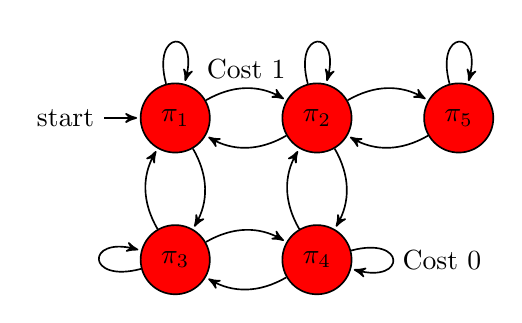
\begin{tikzpicture}[->,>=stealth',shorten >=1pt,auto,node distance=1.8cm,
                    semithick]
  \tikzstyle{every state}=[fill=red,draw=black,text=black]

  \node[initial,state] (A)                    { $\pi_1$};
  \node[state]         (B) [ right of=A] { $\pi_2$};
  \node[state]         (C) [below of=A] { $\pi_3$};
  \node[state]         (D) [right of=C] { $\pi_4$};
  \node[state]         (E) [right of=B] { $\pi_5$};

  \path (A) edge     [bend left]     node {Cost 1}   (B)
  		(B) edge     [bend left]           (A)
		(A) edge     [bend left]         (C)
  		(C) edge     [bend left]           (A)
  		(C) edge     [bend left]         (D)
  		(D) edge     [bend left]           (C)
  		(B) edge     [bend left]           (D)
  		(D) edge     [bend left]           (B)
  		(B) edge     [bend left]           (E)
  		(E) edge     [bend left]           (B)
        (A) edge [loop above]   (A)
        (B) edge [loop above]   (B)
        (C) edge [loop left]   (C)
        (D) edge [loop right]  node {Cost 0} (D)
        (E) edge [loop above]  (E);
\end{tikzpicture}
\end{figure}
\end{frame}

\begin{frame}{B\"uchi Automaton}
\begin{block}{B\"uchi Automaton}
	\small A B\"uchi automaton is a tuple $\mathcal{A}_\varphi = (\mathcal{Q},2^{AP},\delta,\mathcal{Q}_0,\mathcal{F})$ where $\mathcal{Q}$ is a finite set of states, $\mathcal{Q}_0 \subseteq \mathcal{Q}$ is the set of initial states, $2^{AP}$ is the alphabet, $\delta: \mathcal{Q} \times 2^{AP} \rightarrow 2^\mathcal{Q}$ is a transition relation, and $\mathcal{F} \subseteq \mathcal{Q}$ is the set of accepting states.
	\end{block}

	\begin{itemize}
	\item {
	A path on a B\"uchi automaton is accepting if it passes through an accepting state infinitely many times.
	}
	\item {
	For any LTL formula $\varphi$ over $AP$, there exists a B\"uchi automaton over $2^{AP}$ corresponding to $\varphi$ \cite{baier08}
	}
	\end{itemize}
	Reachability while avoiding regions $\varphi = \neg \pi_4 \U \pi_5$
	
	\begin{figure}
\centering
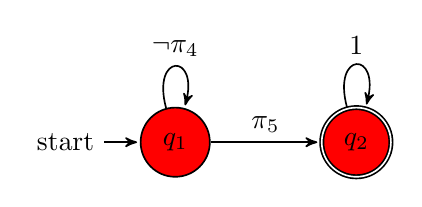
\begin{tikzpicture}[->,>=stealth',shorten >=1pt,auto,node distance=2.3cm,
                    semithick]
  \tikzstyle{every state}=[fill=red,draw=black,text=black]

  \node[initial,state] (A)                    {$q_1$};
  \node[state,accepting]         (B) [right of=A] {$q_2$};

  \path (A) edge              node {$\pi_{5}$} (B)
  		(A) edge [loop above] node {$\neg \pi_4 $} (A)
  		(B) edge [loop above] node {$1$} (B);
\end{tikzpicture}
\end{figure}
\end{frame}

\begin{frame}{Product Automaton}
\begin{block}{Product Automaton}
	\small $\mathcal{A}_p = \mathcal{T}_w \otimes \mathcal{A}_\varphi = (Q', \delta', Q_0', \mathcal{F}', W_p)$, where $Q' = \Pi \times Q = \{ \langle \pi, q \rangle \in Q' | \forall \pi \in \Pi, \hspace{0.2cm} \forall q \in Q \}$; $\delta': Q' \rightarrow 2^{Q'}$. $\langle \pi_j, q_n \rangle \in \delta' (\langle \pi_i, q_m \rangle )$ iff $(\pi_i , \pi_j ) \in \rightarrow_c$ and $q_n \in \delta (q_m, L_d(\pi_j))$; $Q_0' = \{ \langle \pi , q \rangle | \pi \in \Pi_0, \hspace{0.2cm} q_0 \in Q_0\}$, $\mathcal{F}' = \{ \langle \pi, q \rangle | \pi \in \Pi, q \in \mathcal{F}\}$ 
	\end{block}

	\begin{itemize}
	\item {
	Also a B\"uchi automaton
	}
	\end{itemize}
	\begin{figure}
	
\centering
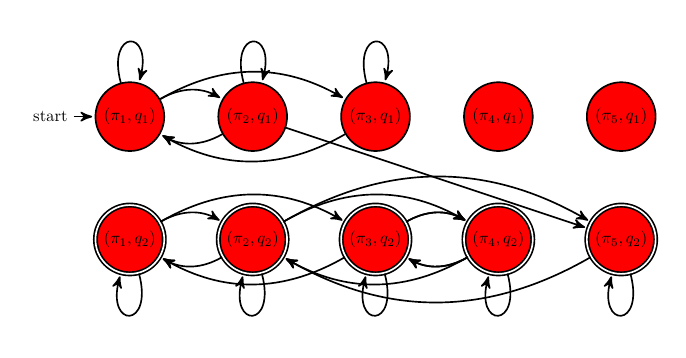
\begin{tikzpicture}[->,>=stealth',shorten >=1pt,auto,node distance=2.6cm,
                    semithick,scale=0.6, every node/.style={transform shape}]
  \tikzstyle{every state}=[fill=red,draw=black,text=black]

  \node[initial,state] (A)                    {$(\pi_1,q_1)$};
  \node[state]         (B) [ right of=A] {$(\pi_2,q_1)$};
  \node[state]         (C) [right of=B] {$(\pi_3,q_1)$};
  \node[state]         (D) [right of=C] {$(\pi_4,q_1)$};
  \node[state]         (E) [right of=D] {$(\pi_5,q_1)$};
  
  \node[state,accepting] 		   (AA)  [below of=A]  {$(\pi_1,q_2)$};
  \node[state,accepting]         (BB) [ right of=AA] {$(\pi_2,q_2)$};
  \node[state,accepting]         (CC) [right of=BB] {$(\pi_3,q_2)$};
  \node[state,accepting]         (DD) [right of=CC] {$(\pi_4,q_2)$};
  \node[state,accepting]         (EE) [right of=DD] {$(\pi_5,q_2)$};  

  \path (A) edge     [bend left]          (B)
        (B) edge     [bend left]          (A)
        (A) edge     [bend left]         (C)
        (C) edge     [bend left]          (A)
        %(C) edge     [bend left]          (D)
        %(D) edge     [bend left]          (C)
		%(B) edge     [bend left]          (D)
        %(D) edge     [bend left]          (B)
        (B) edge               (EE)
        (DD) edge       [bend left]        (BB)
        (BB) edge        [bend left]       (DD)
        (BB) edge        [bend left]       (AA)
        (AA) edge        [bend left]       (BB)
        (BB) edge        [bend left]       (EE)
        (EE) edge        [bend left]       (BB)
        (DD) edge       [bend left]        (CC)
        (CC) edge        [bend left]       (DD)
        (CC) edge        [bend left]       (DD)
        (DD) edge        [bend left]       (CC)
        (CC) edge        [bend left]       (AA)
        (AA) edge        [bend left]       (CC)
        (A) edge [loop above]  (A)
        (B) edge [loop above]  (B)
        (C) edge [loop above]   (C)
        %(D) edge [loop above]   (D)
        (AA) edge [loop below]  (AA)
        (BB) edge [loop below]  (BB)
        (CC) edge [loop below]  (CC)
        (DD) edge [loop below]   (DD)
        (EE) edge [loop below]   (EE);
\end{tikzpicture}

\end{figure}
\end{frame}

\begin{frame}{State-Space Explosion Problem}
\begin{itemize}
\item State-space explosion problem is the is the combinatorial explosion of the number of states in the product automaton.
\item Number of states in B\"uchi automaton can be exponential in the size of the LTL formula \cite{giannakopoulou02} and $|\Q'| = |\Pi|\cdot |\Q|$ 
\item State-space explosion problem is the bottle neck of formal methods based control synthesis.
\end{itemize}
\end{frame}

\subsection{Execution: Path Finding}
\begin{frame}{Accepted Algorithm}
\begin{itemize}
\item {
	We prefer a prefix, suffix structure $R = \langle R_{pre}, R_{suf} \rangle = q_0' q_1' \dots {\color{red} q_f'} [ {\color{red} q_f'} q_{f+1}' \dots q_n']^\omega$ 
}
\end{itemize}
Here is the algorithm currently used in the literature \cite{guo15},\cite{fainekos09},\cite{kloetzer08},\cite{smith2010}
\begin{algorithm}[H]
\caption{OptRun() \cite{guo15}}
\begin{algorithmic}[1]
\Require Input $\A_p$
\Ensure $R_{opt}$
%\Procedure{MyProcedure}{}
%\State If $Q_0'$ or $\F'$ is empty, construct $Q_0'$ or $\F'$ first.
\State For initial state $q_0' \in \Q_0'$, find the optimal path to each $q_f' \in \F$.
\State For each accepting state $q_f' \in \F'$, calculate the optimal path back to $q_f'$. 
\State Find the pair of $(q_{0,opt}',q_{f,opt}')$ that minimizes the total cost
\State Optimal accepting run $R_{opt}$, prefix: shortest path from $q_{0*}'$ to  $q_{f*}$; suffix: the shortest cycle from $q_{f*}'$ and back to itself.
\end{algorithmic}
\end{algorithm}
\end{frame}

% Placing a * after \section means it will not show in the
% outline or table of contents.
\section{Our Contribution}
\subsection{B\"uchi Distance and Algorithm}
\begin{frame}{B\"uchi Distance Measure}  
  \begin{itemize}
  \item {
    We introduce a discrete B\"uchi distance measure, which is the least number of transitions possible to get to an accepting state 
    \pause
    }
  \end{itemize}
  Ex. Sequencing $  \diamond(\pi_3 \land \diamond \pi_5)$
  \begin{figure}
\centering
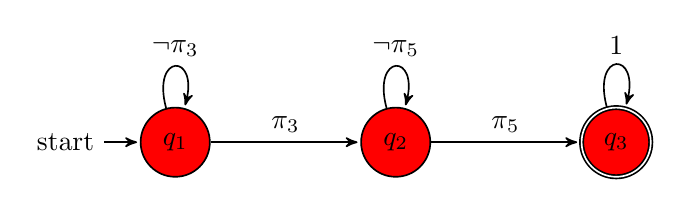
\begin{tikzpicture}[->,>=stealth',shorten >=1pt,auto,node distance=2.8cm,
                    semithick]
  \tikzstyle{every state}=[fill=red,draw=black,text=black]

  \node[initial,state] (A)                    {$q_1$};
  %\node[state] (B)                    [right of=A]{$q_2$};
  \node[state] (B)                    [right of=A]{$q_2$};
  \node[state,accepting]         (C) [right of=B] {$q_3$};

  \path (A) edge              node {$\pi_{3}$} (B)
  		(A) edge [loop above] node {$\neg \pi_3$} (A)
  		(B) edge [loop above] node {$\neg \pi_5$} (B)
  		(B) edge              node {$\pi_{5}$} (C)
  		(C) edge [loop above] node {$1$} (C);
%  		(C) edge              node {$\pi_{3}$} (D)
 % 		(D) edge [loop above] node {$1$} (D);
\end{tikzpicture}
\end{figure}
\pause
\begin{figure}
\centering
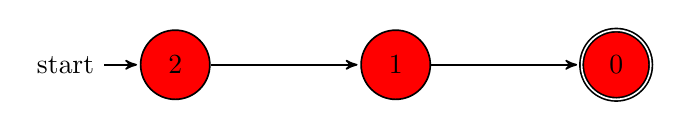
\begin{tikzpicture}[->,>=stealth',shorten >=1pt,auto,node distance=2.8cm,
                    semithick]
  \tikzstyle{every state}=[fill=red,draw=black,text=black]

  \node[initial,state] (A)                    {$2$};
  %\node[state] (B)                    [right of=A]{$q_2$};
  \node[state] (B)                    [right of=A]{$1$};
  \node[state,accepting]         (C) [right of=B] {$0$};

  \path (A) edge               (B)
  		%(A) edge [loop above] node {$\neg \pi_3$} (A)
  		%(B) edge [loop above] node {$\neg \pi_5$} (B)
  		(B) edge              (C);
  		%(C) edge [loop above] node {$1$} (C);
%  		(C) edge              node {$\pi_{3}$} (D)
 % 		(D) edge [loop above] node {$1$} (D);
\end{tikzpicture}
\end{figure}
  \begin{itemize}
  \item {
    Denoted $d_p:\Q \rightarrow \mathbb{Z}$, e.g.\ $d_p(q_2) = 1$ 
    }
  \end{itemize}
\small Note: Transitions with \&\& are removed from LTL2BA because regions do not overlap

\end{frame}




\begin{frame}{Our Algorithm}
\begin{itemize}
\item {
	Motivation for our algorithm: $\mathcal{F}' = \{ \langle \pi, q \rangle | \pi \in \Pi, q \in \mathcal{F}\}$  
}
\item { 
	We greedily find the optimal path which reduces the B\"uchi distance at each step
	}
\end{itemize}
\begin{algorithm}[H]
\caption{GreedyRun()}
\begin{algorithmic}[1]
\Require Input $\A_{p,d}$
\Ensure $R_{g}$
%\Procedure{MyProcedure}{}
\State LEVEL = $d_p(q_0' \in \Q_0')$
\While {LEVEL $> 0$}
\State find optimal path down to $q_n'$ s.t. $d_p(q_n')==LEVEL-1$
\State Level = Level - 1	
\EndWhile
\State Find optimal path from $q_n'$ back to itself
\State Accepting run $R_{g}$, prefix: the optimal paths calculated in the while loop concatenated together; suffix: optimal path from $q_n'$ back to itself.
\end{algorithmic}
\end{algorithm}

\end{frame}

\begin{frame}{Why?}
\begin{itemize}
\item {
	\Large \textbf{We approximate the globally optimal path with a series of locally optimal paths}
}
\item {
	\Large \textbf{We sacrifice a degree of optimality for easier computation!}
}
\end{itemize}
\end{frame}

\begin{frame}{Code}
\begin{itemize}
\item The code for the accepted algorithm is from the P\_MAS\_TG GitHub Repository \cite{pMasGit}.
\item The code for our algorithm is a modified version of code from P\_MAS\_TG.
\item All computations were done on a 2.5 GHz MacBook Pro and used Python 2.7.5.
\end{itemize}


\end{frame}
\section{Performance on Common Formulas}
\subsection{Workspace}
\begin{frame}{Workspace}
\begin{figure}[!htb]
\centering
\includegraphics[scale=0.7]{../writing/workspace.eps}
\label{fig:workspace}
\caption{Workspace 1}
\end{figure}
\end{frame}

\subsection{Reachability While Avoiding Regions}
\begin{frame}[fragile]
\begin{figure}
\centering
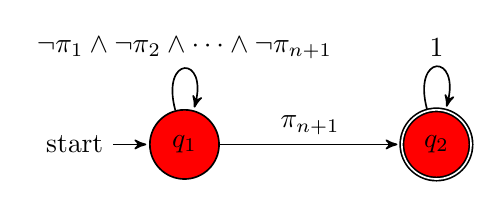
\begin{tikzpicture}[->,>=stealth',shorten >=1pt,auto,node distance=3.2cm,
                    semithick]
  \tikzstyle{every state}=[fill=red,draw=black,text=black]

  \node[initial,state] (A)                    {$q_1$};
  \node[state,accepting]         (B) [right of=A] {$q_2$};

  \path (A) edge              node {$\pi_{n+1}$} (B)
  		(A) edge [loop above] node {$\neg \pi_1 \wedge \neg \pi_2 \wedge \dots \wedge \neg \pi_{n+1}$} (A)
  		(B) edge [loop above] node {$1$} (B);
\end{tikzpicture}
\caption{B\"{u}chi automaton corresponding to $\neg (\pi_1 \lor \pi_2 \lor \dots \pi_n) \U \pi_{n+1}$}
\end{figure}
\centering $d_p(q_1)=1$ and $d_p(q_2)=0$

\begingroup
\fontsize{9pt}{12pt}\selectfont
\begin{lstlisting}
Accepted Algorithm
==================
plan done within 0.02s: precost 37.00, sufcost 0.00
...
full construction and synthesis done within 0.11s
\end{lstlisting}
\endgroup
\begingroup
\fontsize{9pt}{12pt}\selectfont
\begin{lstlisting}
Our Algorithm
==================
plan done within 0.01s: precost 37.00, sufcost 0.00
...
full construction and synthesis done within 0.10s 
\end{lstlisting}
\endgroup
%%% CHECK THIS OUR ALGORITHM SAID .32s



\end{frame}

\begin{frame}{Animation}
asdf
\end{frame}

\subsection{Sequencing}

\begin{frame}
\begin{itemize}
	\item {
	We look at the sequencing formula $\diamond (\pi_1 \land \diamond(\pi_2 \land \diamond \pi_3))$
	}
\end{itemize}
\begin{figure}
\centering
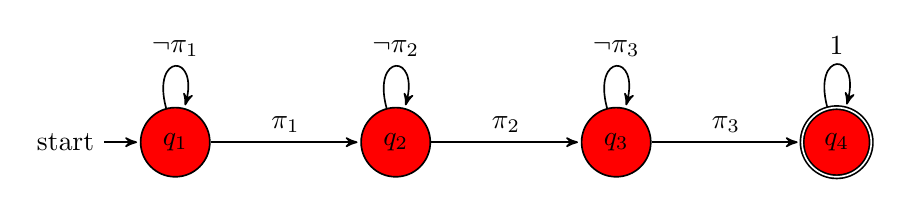
\begin{tikzpicture}[->,>=stealth',shorten >=1pt,auto,node distance=2.8cm,
                    semithick]
  \tikzstyle{every state}=[fill=red,draw=black,text=black]

  \node[initial,state] (A)                    {$q_1$};
  %\node[state] (B)                    [right of=A]{$q_2$};
  \node[state] (B)                    [right of=A]{$q_2$};
  \node[state]         (C) [right of=B] {$q_3$};
  \node[state,accepting]         (D) [right of=C] {$q_4$};

  \path (A) edge              node {$\pi_{1}$} (B)
  		(A) edge [loop above] node {$\neg \pi_1$} (A)
  		(B) edge [loop above] node {$\neg \pi_2$} (B)
  		(B) edge              node {$\pi_{2}$} (C)
  		(C) edge [loop above] node {$\neg \pi_3$} (C)
  		(C) edge              node {$\pi_{3}$} (D)
  		(D) edge [loop above] node {$1$} (D);
\end{tikzpicture}
%\caption{B\"uchi Automaton Corresponding to $  \diamond(\pi_1 \land \diamond (\pi_2 \land \diamond \pi_3))$}
\end{figure}
\begin{itemize}
	\item {
	$d_p(q_1)=3$, $d_p(q_2)=2$, $d_p(q_3)=1$, $d_p(q_4)=0$
	}	
	\item {
	Only one path down $\rightarrow$ Both algorithms calculate the same path!
	}
\end{itemize}
\end{frame}

\begin{frame}[fragile]{Simulation}
\begingroup
\fontsize{9pt}{12pt}\selectfont
\begin{lstlisting}
Accepted Algorithm
==================
plan done within 0.04s: precost 62.00, sufcost 0.00
...
full construction and synthesis done within 0.19s 
\end{lstlisting}
\endgroup
Our algorithm computed the same path, with an output of

\begin{lstlisting}
Our Algorithm
==================
plan done within 0.02s: precost 62.00, sufcost 0.00
...
full construction and synthesis done within 0.17s 
\end{lstlisting}
\end{frame}

\begin{frame}{Nodes Searched}
\begin{figure}[!htb]
\centering
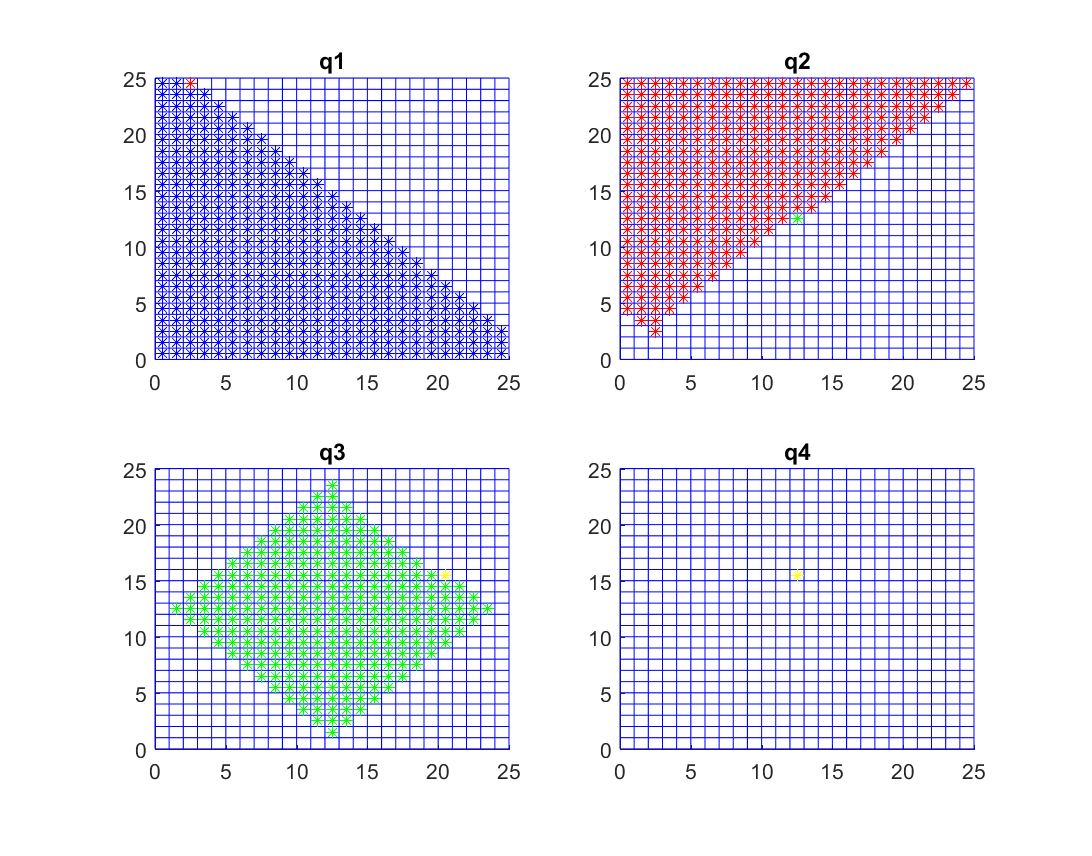
\includegraphics[scale=0.17]{../writing/ourPlot}
\label{fig:animOur}
\caption{Nodes searched with our Algorithm}
\end{figure}

\begin{figure}[!htb]
\centering
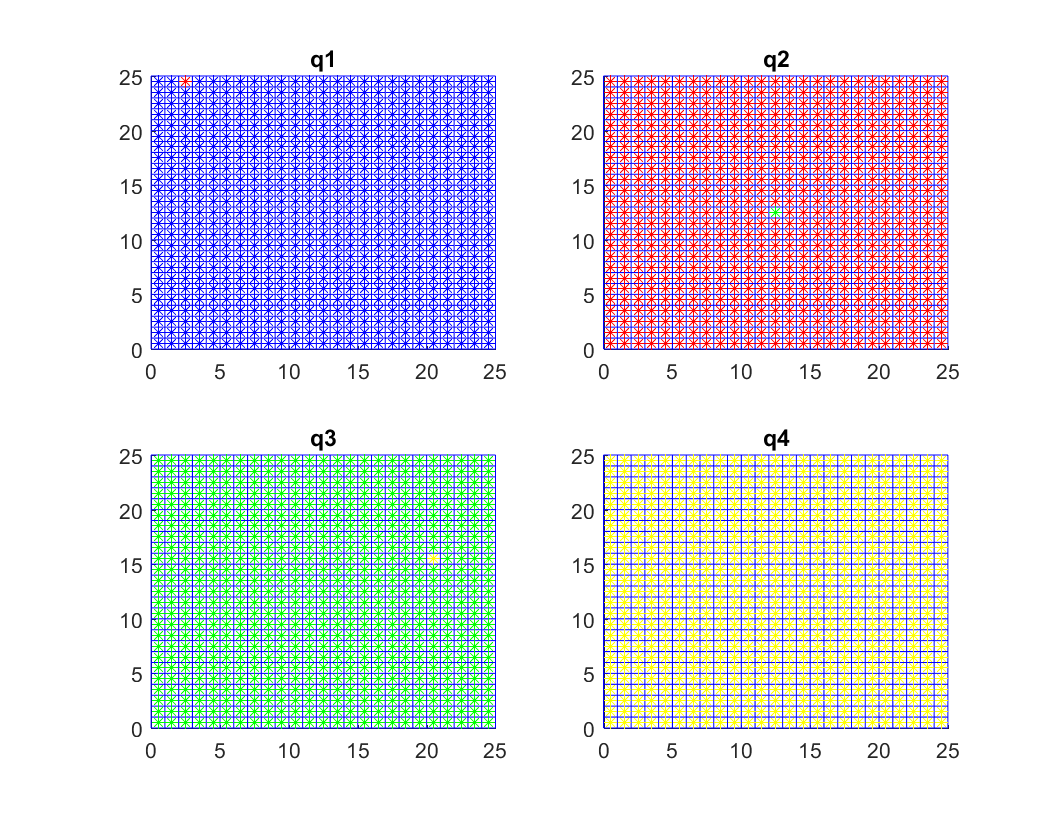
\includegraphics[scale=0.17]{../writing/acceptedPlot}
\label{fig:animAccept}
\caption{Nodes searched with the accepted Algorithm}
\end{figure}
\end{frame}
\subsection{Coverage}
\begin{frame}{Coverage}
\begin{itemize}
\item $\varphi = \diamond \pi_1 \wedge \diamond \pi_2 \wedge \dots \wedge \diamond \pi_n$.
\item A coverage formula represents the statement visit $\pi_1, \pi_2, \dots, \pi_n$ in any order. Ex. $\varphi = \diamond \pi_1 \wedge \diamond \pi_2 \wedge \pi_3$
\end{itemize}
\pause
\begin{figure}
\centering
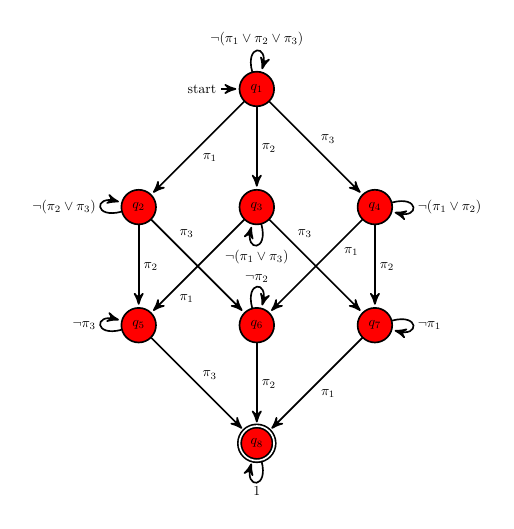
\begin{tikzpicture}[->,>=stealth',shorten >=1pt,auto,node distance=3cm,
                    semithick,scale=0.5, every node/.style={transform shape}]
  \tikzstyle{every state}=[fill=red,draw=black,text=black]

  \node[initial,state] (A)                    {$q_1$};
  \node[state] (C)                    [below of=A]{$q_3$};
  \node[state] (D)                    [right of=C]{$q_4$};
  \node[state]         (B) [left of=C] {$q_2$};
  \node[state] (E) 					[below of=B]{$q_5$};
   \node[state] (F) 					[below of=C]{$q_6$};
   \node[state] (G) 					[below of=D]{$q_7$};
   \node[accepting,state] (H) 					[below of=F]{$q_8$};
  

  \path (A) edge              node {$\pi_{1}$} (B)
   (A) edge              node {$\pi_{2}$} (C)
   (A) edge              node {$\pi_{3}$} (D)
   (B) edge              node {$\pi_{2}$} (E)
   (B) edge              node [near start] {$\pi_{3}$} (F)
   (C) edge              node [near end] {$\pi_{1}$} (E)
   (E) edge              node {$\pi_{3}$} (H)
   (F) edge              node {$\pi_{2}$} (H)
   (G) edge              node {$\pi_{1}$} (H)
   (D) edge              node {$\pi_{2}$} (G)
   (A) edge      [loop above]        node {$\neg (\pi_1 \lor \pi_{2} \lor\pi_3)$} (A)
   (B) edge      [loop left]        node {$\neg (\pi_{2} \lor \pi_3)$} (B)
   (C) edge      [loop below]        node {$\neg( \pi_1 \lor \pi_3)$} (C)
   (D) edge      [loop right]        node {$\neg (\pi_1 \lor \pi_{2}) $} (A)
   (E) edge      [loop left]        node {$\neg  \pi_3$} (E)
   (F) edge      [loop above]        node {$\neg  \pi_2$} (F)
   (G) edge      [loop right]        node {$\neg  \pi_1$} (G)
   (H) edge      [loop below]        node {$1$} (H)
   (D) edge              node [near start] {$\pi_{1}$} (F)
   (C) edge              node [near start] {$\pi_{3}$} (G);
\end{tikzpicture}
%\caption{B\"uchi Automaton Corresponding to $\diamond \pi_1 \wedge \diamond \pi_2 \wedge \diamond \pi_3$}
\end{figure}
\end{frame}

\begin{frame}{Coverage}
\begin{figure}
\centering
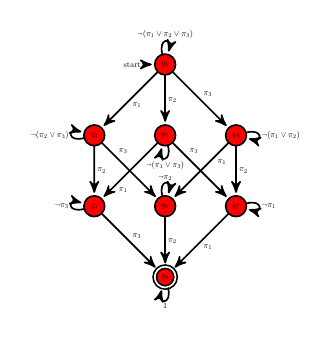
\begin{tikzpicture}[->,>=stealth',shorten >=1pt,auto,node distance=3cm,
                    semithick,scale=0.3, every node/.style={transform shape}]
  \tikzstyle{every state}=[fill=red,draw=black,text=black]

  \node[initial,state] (A)                    {$q_1$};
  \node[state] (C)                    [below of=A]{$q_3$};
  \node[state] (D)                    [right of=C]{$q_4$};
  \node[state]         (B) [left of=C] {$q_2$};
  \node[state] (E) 					[below of=B]{$q_5$};
   \node[state] (F) 					[below of=C]{$q_6$};
   \node[state] (G) 					[below of=D]{$q_7$};
   \node[accepting,state] (H) 					[below of=F]{$q_8$};
  

  \path (A) edge              node {$\pi_{1}$} (B)
   (A) edge              node {$\pi_{2}$} (C)
   (A) edge              node {$\pi_{3}$} (D)
   (B) edge              node {$\pi_{2}$} (E)
   (B) edge              node [near start] {$\pi_{3}$} (F)
   (C) edge              node [near end] {$\pi_{1}$} (E)
   (E) edge              node {$\pi_{3}$} (H)
   (F) edge              node {$\pi_{2}$} (H)
   (G) edge              node {$\pi_{1}$} (H)
   (D) edge              node {$\pi_{2}$} (G)
   (A) edge      [loop above]        node {$\neg (\pi_1 \lor \pi_{2} \lor\pi_3)$} (A)
   (B) edge      [loop left]        node {$\neg (\pi_{2} \lor \pi_3)$} (B)
   (C) edge      [loop below]        node {$\neg( \pi_1 \lor \pi_3)$} (C)
   (D) edge      [loop right]        node {$\neg (\pi_1 \lor \pi_{2}) $} (A)
   (E) edge      [loop left]        node {$\neg  \pi_3$} (E)
   (F) edge      [loop above]        node {$\neg  \pi_2$} (F)
   (G) edge      [loop right]        node {$\neg  \pi_1$} (G)
   (H) edge      [loop below]        node {$1$} (H)
   (D) edge              node [near start] {$\pi_{1}$} (F)
   (C) edge              node [near start] {$\pi_{3}$} (G);
\end{tikzpicture}
%\caption{B\"uchi Automaton Corresponding to $\diamond \pi_1 \wedge \diamond \pi_2 \wedge \diamond \pi_3$}
\end{figure}
\begin{itemize}
\item Now we have "choices" that have to be made!
\item Choices $\rightarrow$ we lose optimality. The path our algorithm finds will likely cost more than the path calculated by the accepted algorithm. However our path is computed faster.
\end{itemize}
\end{frame}

\begin{frame}[fragile]{Coverage}
\begingroup
\fontsize{9pt}{12pt}\selectfont
\begin{lstlisting}
Accepted Algorithm
==================
plan done within 0.08s: precost 59.00, sufcost 0.00
...
full construction and synthesis done within 0.43s 
\end{lstlisting}
\endgroup
and our algorithm is 

\begingroup
\fontsize{9pt}{12pt}\selectfont
\begin{lstlisting}
Our Algorithm
==================
plan done within 0.02s: precost 62.00, sufcost 0.00
...
full construction and synthesis done within 0.38s 
\end{lstlisting}
\endgroup
\end{frame}

\begin{frame}{Cost Bound}
\begin{itemize}
\item The travelling salesperson problem: "Given a list of cities and the distances between each pair of cities, what is the shortest possible route that visits each city exactly once and returns to the origin city?"
\item It has been shown \cite{rosenkrantz74} that for an n-node travelling salesperson problem which satisfies the triangle inequality
\begin{align*}
\text{NEARNEIBR} \leq (\frac{1}{2} \lceil \log(n) \rceil + \frac{1}{2})\text{OPTIMAL}
\end{align*}
\item \cite{lenstra75} shows how to formulate seeming unrelated problems as travelling salesperson problems by introducing a dummy node.
\item We introduce a dummy node * which is $\max_{i,j} c_{i,j}$ where $c_{i,j}$ is the cost from $\pi_i$ to $\pi_j$.
\item Then our bound is  
\begin{align*}
\text{GREEDY} + 2\max_{i,j} c_{i,j} \leq (\frac{1}{2} \lceil \log(n) \rceil + \frac{1}{2}) (\text{ACCEPT} + 2 \max_{i,j} c_{i,j}) \\ 
\end{align*}
\end{itemize}
\end{frame}

\subsection{Recurrence (Liveness)}
\begin{frame}{Recurrence (Liveness)}
\begin{figure}
\centering
\begin{itemize}
\item Recurrence: "Visit $\pi_1$, $\pi_2$, $\dots$, $\pi_n$ infinitely many times."
\end{itemize}
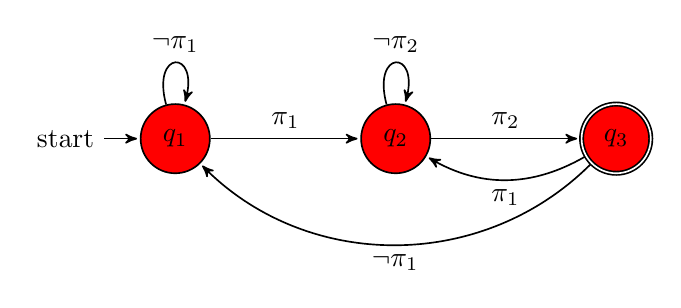
\begin{tikzpicture}[->,>=stealth',shorten >=1pt,auto,node distance=2.8cm,
                    semithick]
  \tikzstyle{every state}=[fill=red,draw=black,text=black]

  \node[initial,state] (A)                    {$q_1$};
  \node[state] (B)                    [right of=A]{$q_2$};
  \node[state,accepting] (C)                    [right of=B]{$q_3$};

  \path (A) edge              node {$\pi_{1}$} (B)
  		(A) edge [loop above] node {$\neg \pi_1$} (A)
  		(B) edge [loop above] node {$\neg \pi_2$} (B)
  		(B) edge              node {$\pi_{2}$} (C)
  		(C) edge [bend left=45] node {$\neg \pi_1$} (A)
  		(C) edge  [bend left] node {$\pi_{1}$} (B);
%  		(D) edge [bend right] node {$\neg \pi_1$} (A)
 % 		(D) edge [bend left] node {$\pi_1$} (B);
\end{tikzpicture}
\caption{B\"uchi Automaton for $\ssquare(\diamond \pi_1 \land \diamond \pi_2 )$ 1}
\label{fig:gasBuchiRec}
\end{figure}
\begin{itemize}
\item \small Automaton from LTL2BA. Note: Not tight.
\pause
\item For the first time we have a formula that has a \textbf{non-trivial suffix}.
\end{itemize}
\end{frame}

\begin{frame}[fragile]{Case Study}
\begin{itemize}
\item Remember that the accepted algorithm computes the suffix from \textbf{every} accepting state. That implies a lot of work for this formula.
\end{itemize}
\pause
\begingroup
\fontsize{9pt}{12pt}\selectfont
\begin{lstlisting}
Accepted Algorithm
==================
plan done within 16.17s: precost 62.00, sufcost 60.00
------------------------------
...
full construction and synthesis done within 16.35s 
\end{lstlisting}
\endgroup
while our algorithm did it in
\begingroup
\fontsize{9pt}{12pt}\selectfont
\begin{lstlisting}
Our Algorithm
==================
plan done within 0.04s: precost 62.00, sufcost 60.00
------------------------------
...
full construction and synthesis done within 0.21s 
\end{lstlisting}
\endgroup
\end{frame}

\section{More Complex Formulas}
\subsection{Study of Various Formulas}
\begin{frame}{Analysis}
\begin{itemize}
\item More complex formulas prove difficult to analyze because the B\"uchi automaton becomes very big and cannot be visualized. 
\item Took formulas from \cite{somenzi00} to show extensive and non-biased experimentation.
\end{itemize}
\begin{table}[]
\centering
\small
\scalebox{0.6}{
\begin{tabular}{|c|c|c|c|c|}
\hline
Formula & \makecell{Accepted Cost \\ prefix, suffix} & Accepted Time & \makecell{Our Cost \\ prefix, suffix} & Our Time \\ \hline
     '(!r223 U r445) $||$ (!r268 U r435)'  &         27 ,0     &      0.04         &      27,0   &     0.01     \\ \hline
      '!r62 U(!r266 U r422)'  &         38.00 ,0     &       0.05        &     38,0     &     0.02     \\ \hline
       '[]$<>$ r0 $->$ []$<>$ r317' &         1,0      &       5.06        &    1,0      &    0.00     \\ \hline
       '[]$<>$ r0 $<->$ []$<>$ r317'  & 1,0		&		10.70		& 1,0 	&  0.00 \\ \hline 
      '!($<><>$ r498 $<->$ r541)' &	42.00	&	0.03	&	42.00	&	0.02	\\		\hline
      '!([]$<>$ r3 $->$ []$<>$r591)' &	 3.00, 0	&	5.06 	&	3.00, 0 	&	0.00	\\		\hline
      '!([]$<>$ r3 $<->$ []$<>$r591)' &	 3.00, 0	&	10.31	&	39, 0	&	0.01	\\		\hline
      '!r532 R (!r432 || r321)' &	 0,0	&	4.97 	&	0,0	&	0.01 	\\		\hline
     \makecell{ '$<>$ r114 \&\& [](r114 $-> <>$ r12) \&\& \\((X r114 U X r12) $||$ !X( r114 U r12))' }&	24.00	&	0.08 	&	24.00	&	0.01	\\		\hline
   \makecell{ '$<>$ pickrball \&\& [](pickrball $-> <>$ droprball) \\ \&\& ((X pickrball U X droprball) $||$ !X( pickrball U droprball))' } &	47.00,0	&	28.87	&	47.00,0	&	0.03	\\		\hline
      ' $<>$ r124 \&\& $<>$ !r124' &	28.00,0	&	0.05 	&	28.00,0	&	0.01	\\		\hline
%      &		&		&		&		\\		\hline
 %     &		&		&		&		\\		\hline
  %    &		&		&		&		\\		\hline
\end{tabular}}
\caption{Comparison of Accepted Algorithm with Our Algorithm on Various Examples}
\label{table}
\end{table}
\end{frame}


\section{Conclusions}
\begin{frame}{Benefits}
\begin{itemize}
\item Works very well on reachability while avoiding regions, sequencing, and recurrence (when the automaton is not tight). Guaranteed to get the same path faster!
\item Saves a lot of time when the formula does not have a trivial suffix.
\end{itemize}
\end{frame}

\begin{frame}{Drawbacks}
\begin{itemize}
\item Hard to analyze the performance on more complex formulas.
\item When there is a trivial suffix, the majority of the time is spent on constructing the graph and the search is usually quick. Future work could be to use this algorithm for on-the-fly construction. 
\end{itemize}


\end{frame}


\begin{frame}[allowframebreaks]
	%\begin{thebibliography}{10}
        \frametitle{References}
        \bibliographystyle{amsalpha}
        \bibliography{../writing/bibliography}
     %\end{thebibliography}
\end{frame}

\end{document}